\section{Metadata: Semantics}

\begin{frame}{Day 2 - Part 5: Semantics \& Vocabularies}{10:50 - 11:35}
    \begin{block}{Module 5 Goal}
        It's not enough for machines to \emph{read} data. They must \emph{understand} it. This is \textbf{Semantics}, the core of Interoperability ('I').
    \end{block}
    \begin{center}
        
\includegraphics[width=0.32\textwidth]{figs/fig_d2p5/fig_d2p5_01-semantic}
        \captionof{figure}{Semantics provides shared meaning, like a universal translator.}
    \end{center}
\end{frame}

\begin{frame}{Learning Objectives (5.1)}
    \begin{itemize}
        \item \textbf{List} three examples of knowledge organisation systems (KOS) used in RDM (controlled vocabularies, thesauri, ontologies).
        \item \textbf{Recall} the core components of the \textbf{Protégé} UI for defining classes and properties.
    \end{itemize}
\end{frame}

\begin{frame}{Theory: The Knowledge "Ladder" (KOS)}‚{Module 5.1: List}
    %% \begin{center}
    %%     \includegraphics[width=0.4\textwidth]{example-image-b}
    %% \end{center}
    
    \begin{itemize}
        \item \textbf{1. Controlled Vocabulary (List):}
        \item A simple, flat list of allowed terms. (e.g., `['male', 'female', 'other']`).
        \pause
        \item \textbf{2. Thesaurus (Hierarchy):}
        \item A list with relationships. (e.g., `Karlsruhe` $\rightarrow$ Broader Term: `Baden-Württemberg`).
        \pause
        \item \textbf{3. Ontology (Logical Model):}
        \item A formal model of a domain. (e.g., `Karlsruhe` \emph{is\_a} `City`. A `City` \emph{has\_population} `Integer`. A `City` \emph{is\_located\_in} `State`.)
    \end{itemize}
\end{frame}

\begin{frame}{Theory: Intro to Protégé}{Module 5.1: Recall}
    \textbf{Protégé} is a free, open-source \textbf{ontology editor}. It is the standard tool for building and managing formal ontologies.
    
    \begin{block}{Core Components of Protégé}
        \begin{itemize}
            \item \textbf{Classes:} The "things" or "concepts" in your domain. (e.g., `Experiment`, `Sample`, `Instrument`).
            \pause
            \item \textbf{Object Properties:} Relationships between classes. (e.g., `Experiment` $\rightarrow$ \emph{uses\_instrument} $\rightarrow$ `Instrument`).
            \pause
            \item \textbf{Data Properties:} Relationships from a class to a value. (e.g., `Sample` $\rightarrow$ \emph{has\_weight} $\rightarrow$ `float`).
            \pause
            \item \textbf{Axioms:} The logical rules. (e.g., `Experiment` \emph{must\_have\_at\_least\_one} `Sample`).
        \end{itemize}
    \end{block}
\end{frame}

\begin{frame}{Interactive: Demo Protégé}{Module 5.1: Practice}
    \begin{block}{Live Demo (10 min)}
        \textbf{Task:} Let's open Protégé and look at a simple ontology.
        \pause
        \begin{itemize}
            \item \textbf{Recall:} Where is the 'Classes' tab?
            \item \textbf{Recall:} Where is the 'Object Properties' tab?
            \item We will create one class, `HMC\_Researcher`, and one data property, `has\_ORCID`.
        \end{itemize}
        \pause
        \textbf{Goal:} \textbf{Recall} the core components of the UI.
    \end{block}
\end{frame}

\begin{frame}{Learning Objectives (5.2)}
    \begin{itemize}
        \item \textbf{Explain} how a \textbf{controlled vocabulary} (CV) improves the \textbf{Interoperability} ('I') of a dataset.
        \item \textbf{Explain} how \textbf{LinkML} facilitates the \textbf{Interoperability} of two distinct data models.
    \end{itemize}
\end{frame}

\begin{frame}{Theory: How CVs Enable Interoperability}{Module 5.2: Explain}
    \begin{columns}
        \column{.5\textwidth}
        \begin{block}{Without a CV (Low 'I')}
            \begin{itemize}
                \item `Researcher 1: "temp"`
                \item `Researcher 2: "T"`
                \item `Researcher 3: "temperature"`
            \end{itemize}
            \pause
            A computer search for "temperature" will \textbf{miss} the data from Researchers 1 and 2. The data is not interoperable.
        \end{block}
        
        \column{.5\textwidth}
        \begin{block}{With a CV (High 'I')}
            \textbf{CV:} `MyLab:Temperature` (URI)
            \begin{itemize}
                \item `Researcher 1: MyLab:Temperature`
                \item `Researcher 2: MyLab:Temperature`
                \item `Researcher 3: MyLab:Temperature`
            \end{itemize}
            \pause
            A computer can now search for `MyLab:Temperature` and find \textbf{all three} datasets. They can be automatically combined.
        \end{block}
    \end{columns}
\end{frame}

\begin{frame}{Theory: Intro to LinkML}{Module 5.2: Explain}
    \textbf{LinkML} is a modelling language (written in simple YAML) that helps you \textbf{design} and \textbf{validate} data models.
    \begin{columns}
        \column{.36\textwidth}
        \begin{center}
            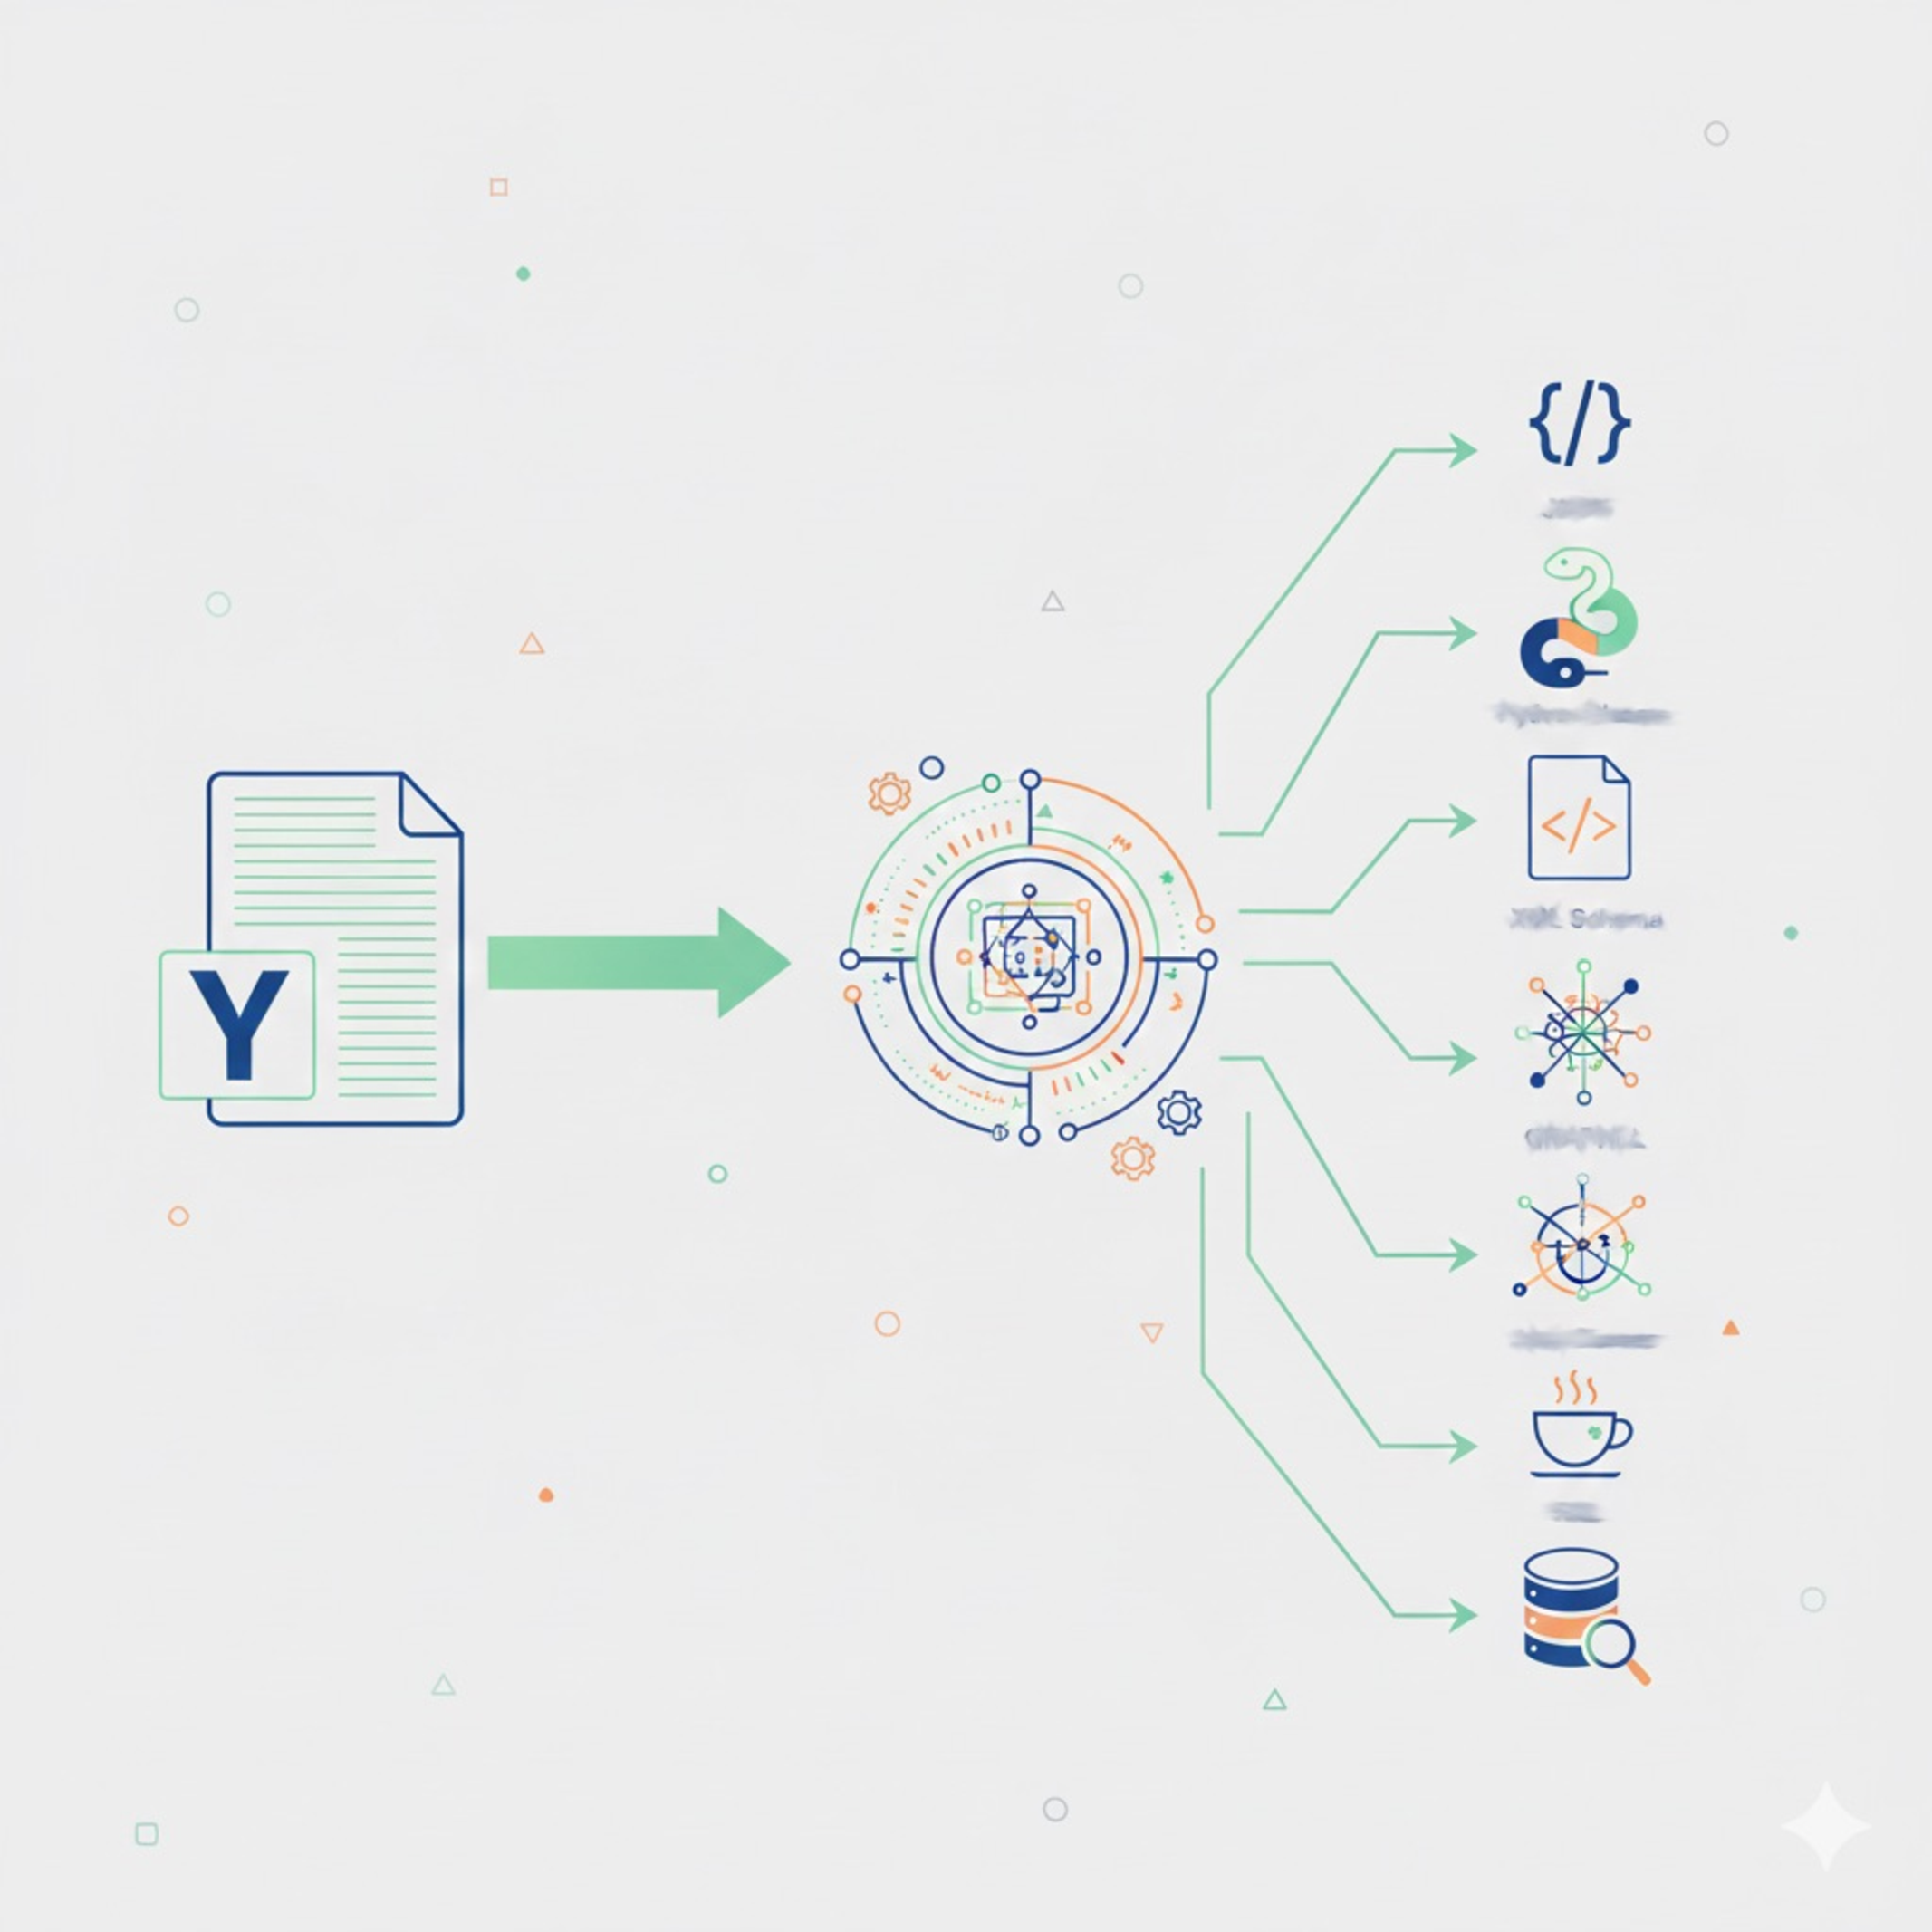
\includegraphics[width=0.8\textwidth]{figs/fig_d2p5/fig_d2p5_02-lnkml}
            \captionof{figure}{One Model $\rightarrow$ Many Formats}
        \end{center}
        \column{.64\textwidth}
        You write one simple `schema.yaml` file...
        \pause
        LinkML \textbf{auto-generates} all of these:
        \begin{itemize}
            \item \textbf{JSON-Schema} (for validation)
            \item \textbf{Python Classes} (for your scripts)
            \item \textbf{XML Schema (XSD)} (for your archive)
            \item \textbf{GraphQL} (for your web API)
        \end{itemize}
        \pause
        It is the \textbf{ultimate} tool for Interoperability ('I').
    \end{columns}
\end{frame}

\begin{frame}{Interactive: The Power of CVs and LinkML}{Module 5.2: Practice}
    \begin{block}{Discussion (10 min)}
        \textbf{Task:}
        \begin{itemize}
            \item \textbf{Explain} in your own words how a CV stops researchers from "making up" metadata terms.
            \pause
            \item \textbf{Explain} how LinkML solves the "XML vs. JSON" problem we had in Module 4. (Answer: It generates \textit{both} from one source!)
        \end{itemize}
        \pause
        \textbf{Goal:} \textbf{Explain} how these tools enable 'I'.
    \end{block}
\end{frame}

\begin{frame}{Learning Objectives (5.3)}
    \begin{itemize}
        \item \textbf{Map} free-text keywords to standardised terms in a \textit{domain-specific thesaurus}.
        \item \textbf{Map} classes and properties between two existing ontologies using \textbf{Protégé}.
    \end{itemize}
\end{frame}

\begin{frame}{Theory: Mapping Free-Text}{Module 5.3: Map}
    Mapping is the process of \emph{translating} your messy, free-text "internal" terms to the clean, public "standard" terms.
    
    \begin{block}{Example: Mapping to a Thesaurus}
        \begin{itemize}
            \item \textbf{Your Term:} "Pressure"
            \pause
            \item \textbf{Thesaurus:} `Gemet`
            \item \textbf{Search "Pressure":} Find `http://.../atmospheric\_pressure`
            \pause
            \item \textbf{Mapping:} Your `pressure` $\rightarrow$ `owl:equivalentClass` $\rightarrow$ `gemet:atmospheric\_pressure`
        \end{itemize}
    \end{block}
    You have now made your data interoperable with everyone else who uses the `Gemet` thesaurus.
\end{frame}

\begin{frame}{Theory: Mapping in Protégé}{Module 5.3: Map}
    Protégé is the tool for mapping two complex \emph{ontologies}.
    
    \textbf{Scenario:}
    \begin{itemize}
        \item `Ontology\_A` (from Biology) has a class: `Human`
        \item `Ontology\_B` (from Medicine) has a class: `Patient`
    \end{itemize}
    \pause
    Are these the same?
    \pause
    \begin{block}{Mapping Axioms in Protégé}
        \begin{itemize}
            \item `Ontology\_A:Human` $\rightarrow$ `owl:equivalentClass` $\rightarrow$ `Ontology\_B:Patient`
            (This means they are identical)
            \pause
            \item `Ontology\_A:Human` $\rightarrow$ `rdfs:subClassOf` $\rightarrow$ `Ontology\_B:Patient`
            (This means all Humans are Patients, but not all Patients are Humans - maybe some Patients are animals?)
        \end{itemize}
    \end{block}
    This logic is the core of semantic interoperability.
\end{frame}

\begin{frame}{Interactive: Mapping Workshop}{Module 5.3: Practice}
    \begin{block}{Workshop: Two Tracks (15 min)}
        \begin{columns}
            \column{.5\textwidth}
            \begin{block}{Track 1: Thesaurus}
                \textbf{Goal:} \textbf{Map} free-text.
                \pause
                \begin{itemize}
                    \item Go to a public thesaurus (e.g., `Gemet`, `AGROVOC`).
                    \item Find a term for "soil".
                    \item Find the URI.
                \end{itemize}
            \end{block}
            
            \column{.5\textwidth}
            \begin{block}{Track 2: Protégé (Demo)}
                \textbf{Goal:} \textbf{Map} two classes.
                \pause
                \begin{itemize}
                    \item (Live Demo)
                    \item Load two simple ontologies.
                    \item Create an `owl:equivalentClass` axiom between two classes.
                \end{itemize}
            \end{block}
        \end{columns}
    \end{block}
\end{frame}

\begin{frame}{Learning Objectives (5.4)}
    \begin{itemize}
        \item \textbf{Assess} a metadata record to \textbf{identify} free-text entries that should be replaced by a CV.
        \item \textbf{Assess} a candidate \textbf{LinkML schema} to \textbf{identify} structural conflicts.
    \end{itemize}
\end{frame}

\begin{frame}[fragile]{Theory: Assessing a Metadata Record}{Module 5.4: Assess}
\begin{columns}
    \column{.5\textwidth}
    \begin{block}{A "Bad" Metadata Record (Free-Text)}
\begin{lstlisting}[language=json]
{
  "title": "My Test",
  "material": "Steel",
  "measurement": "Toughness"
}
\end{lstlisting}
    \end{block}
        
    \column{.5\textwidth}
    \begin{block}{An "Assessed \& Improved" Record (CV)}
\begin{lstlisting}[language=json]
{
  "title": "My Test",
  "material": "emmo:SS-304",
  "measurement": "omat:Charpy_Impact_Test"
}
\end{lstlisting}
    \end{block}
\end{columns}
    \pause
    \textbf{Assessment:}
    \begin{itemize}
        \item What is "Steel"? (Which grade? `SS-304`? `SS-316`?)
        \item What is "Toughness"? (Charpy test? Izod test?)
    \end{itemize}
    \pause

    We \textbf{identified} the free-text and \textbf{replaced} it with URIs from a CV.
\end{frame}

\begin{frame}[fragile]{Theory: Assessing a LinkML Schema}{Module 5.4: Assess}

    \textbf{Problem:} You try to merge two data models (schemas) using LinkML.
    \bigskip
    
    \begin{columns}
        \column{.36\textwidth} 
        \begin{block}{Model A}
            \begin{lstlisting}[language=yaml]
classes:
  Sample:
    slots:
      ID:
        identifier: true
            \end{lstlisting}
        \end{block}
        \pause
        \column{.36\textwidth}
        \begin{block}{Model B}
            \begin{lstlisting}[language=yaml]
classes:
  Specimen:
    slots:
      UUID:
        identifier: true
            \end{lstlisting}
        \end{block}
        
    \end{columns}
    \vfill
    \pause
    \textbf{Assessment:} You have a \textbf{structural conflict}. `Sample` and `Specimen` are probably the same thing (`owl:equivalentClass`), but they have different identifier names (`ID` vs. `UUID`). LinkML helps you \textbf{identify} and \textbf{map} these conflicts.
\end{frame}

\begin{frame}[fragile]{Interactive: Find the Free-Text}{Module 5.4: Practice}
    \begin{block}{Activity (10 min)}
        \textbf{Task:} Look at this "bad" metadata record. \textbf{Assess} it and \textbf{identify} all the ambiguous free-text fields that need to be replaced by a CV.
\begin{lstlisting}[language=json]
{
  "author": "M. Schmidt",
  "date": "Oct 10, 2024",
  "location": "CN, Bldg 301",
  "instrument": "Zeiss Scope",
  "material": "Copper",
  "result": "Good"
}
\end{lstlisting}
        \pause
        \textbf{Answers:} `author` (needs ORCID), `date` (needs ISO format), `location` (needs URI), `instrument` (needs ID), `material` (needs URI), `result` (needs vocab).
    \end{block}
\end{frame}

\begin{frame}{Learning Objectives (5.5)}
    \begin{itemize}
        \item \textbf{Justify} the selection of a specific \textbf{ontology} over a simpler \textbf{controlled vocabulary}.
        \item \textbf{Justify} the decision to use an advanced feature in \textbf{Protégé} (e.g., reasoners).
    \end{itemize}
\end{frame}
\begin{frame}{Theory: CV vs. Ontology}
    \frametitle{Module 5.5: Justify}
    When do you need the complexity of an ontology?
    
    \begin{columns}
        \column{.5\textwidth}
        \begin{block}{Use a Controlled Vocabulary (CV)}
            \textbf{When:} You need to \emph{standardise input}.
            \begin{itemize}
                \item Drop-down lists.
                \item Simple tags.
                \item Harmonising keywords.
            \end{itemize}
            \textbf{Query:} "Find all data tagged with `Karlsruhe`."
        \end{block}
        
        \column{.5\textwidth}
        \begin{block}{Use an Ontology}
            \textbf{When:} You need to ask \emph{complex, logical questions}.
            \begin{itemize}
                \item `Experiment` \emph{uses\_material} `Steel`
                \item `Steel` \emph{has\_component} `Iron`
            \end{itemize}
            \textbf{Query:} "Find all experiments that used a material which has Iron as a component."
        \end{block}
    \end{columns}
    \pause
    \textbf{Justification:} You \textit{must} use an ontology if your research questions require logical inference.
\end{frame}

\begin{frame}{Theory: Protégé Reasoners}{Module 5.5: Justify}
    \begin{columns}
        \column{.36\textwidth}
        \begin{center}
            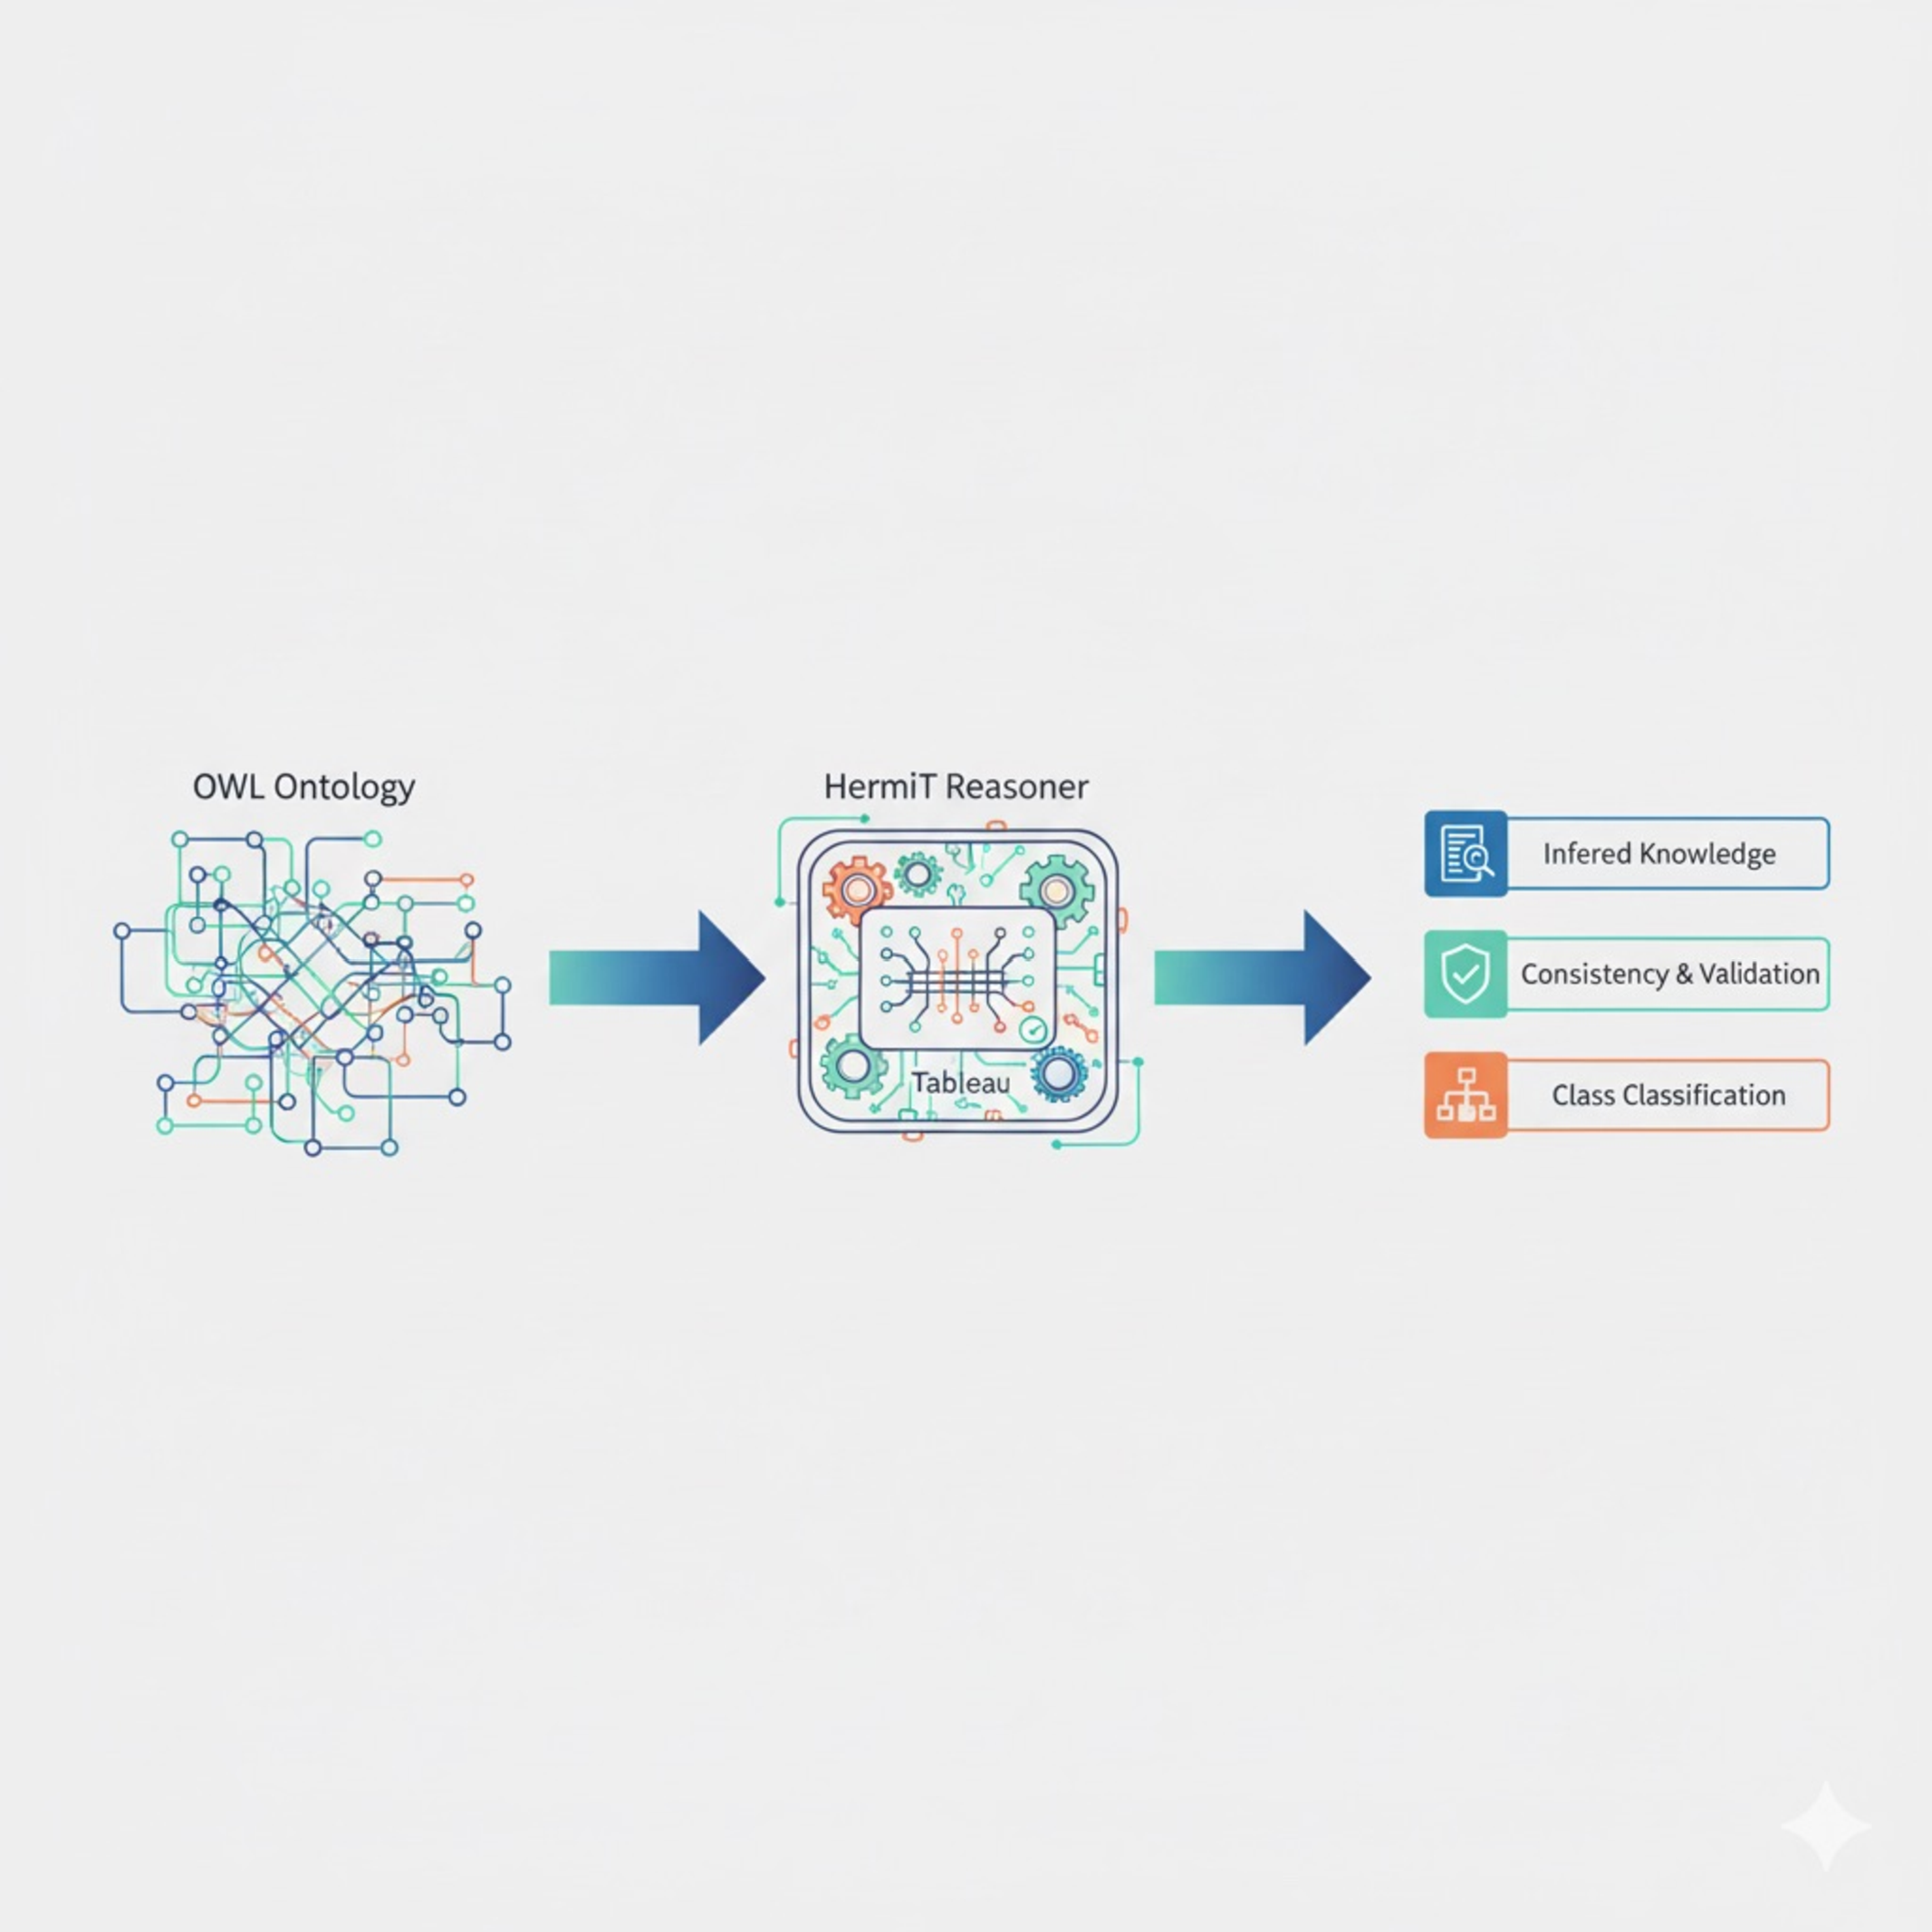
\includegraphics[width=0.8\textwidth]{figs/fig_d2p5/fig_d2p5_03-hermit}
            \captionof{figure}{A reasoner is a "logic engine" for your ontology.}
        \end{center}
        \column{.74\textwidth}
        You state the facts. The reasoner finds the hidden knowledge.
        \pause
        \begin{itemize}
            \item \textbf{You state:} `Karlsruhe` \emph{is\_a} `City`.
            \item \textbf{You state:} `City` \emph{is\_a} `Populated\_Place`.
            \pause
            \item \textbf{Reasoner infers:} `Karlsruhe` \emph{is\_a} `Populated\_Place`. (Transitivity)
        \end{itemize}
        \pause
        \textbf{Justification:} You \textit{must} use a reasoner to \textbf{validate the semantic consistency} of your model. If you state `A` is a `B`, and `B` is a `C`, but also `A` \emph{cannot} be a `C` (disjoint), the reasoner will raise an error and tell you your logic is broken.
            
    \end{columns}
\end{frame}

\begin{frame}{Interactive: Vocab or Ontology?}{Module 5.5: Practice}
    \begin{block}{Scenario (15 min)}
        \textbf{Task:} For each scenario, \textbf{justify} your choice: a simple \textbf{CV} or a full \textbf{Ontology}?
        \pause
        \begin{itemize}
            \item \textbf{Scenario 1:} You want to standardise the "Country" field in a user sign-up form.
            \item \emph{Answer:} \textbf{CV}. (A simple list).
            \pause
            \item \textbf{Scenario 2:} You want to model the entire energy grid, including power plants, substations, and the flow of electricity between them, to find weak points.
            \item \emph{Answer:} \textbf{Ontology}. (Needs complex relationships).
            \pause
            \item \textbf{Scenario 3:} You want to validate that your semantic mappings between two models are logical and not contradictory.
            \item \emph{Answer:} \textbf{Ontology with a Reasoner}.
        \end{itemize}
    \end{block}
\end{frame}
\begin{frame}{Learning Objectives (5.6)}
    \begin{itemize}
        \item \textbf{Develop} a simple, internal \textbf{controlled vocabulary} (CV) for an ELN template.
        \item \textbf{Develop} a \textbf{LinkML data model} that expresses semantic similarities identified via mapping.
    \end{itemize}
\end{frame}

\begin{frame}{Interactive: Draft an Internal CV}{Module 5.6: Practice}
    \begin{block}{Activity (10 min)}
        \textbf{Task:} Let's \textbf{develop} a simple internal CV for our ELN.
        \pause
        \textbf{Field:} `experiment\_status`
        \pause
        \textbf{Brainstorm:} What are the allowed terms?
        \begin{itemize}
            \item `planning`
            \item `active`
            \item `paused`
            \item `completed`
            \item `failed`
        \end{itemize}
        \pause
        \textbf{Result:} You have just created a CV! You can now build this into your ELN as a drop-down list to prevent "free-text" like "done" or "finished".
    \end{block}
\end{frame}

\begin{frame}[fragile]{Interactive: Draft a LinkML Model}{Module 5.6: Practice}
    \begin{block}{Challenge: Draft a LinkML Model (15 min)}
        \textbf{Task:} Remember our mapping: `Model A: Sample` and `Model B: Specimen`. \\
        \pause
        \textbf{Goal:} \textbf{Develop} a LinkML model that merges them. \\
        \pause
        \textbf{Solution (YAML):}
        \begin{columns}
            \column{.36\textwidth}
\begin{lstlisting}[language=yaml]
classes:
  MyMergedClass:
    # We map to BOTH ontologies
    is_a: ModelA:Sample
    exact_mappings:
      - ModelB:Specimen
    slots:
      # We merge the slots
      - ID
      - UUID
\end{lstlisting}

        \end{columns}
        \pause
        This LinkML model now formally expresses the semantic similarity.
    \end{block}
\end{frame}

\begin{frame}{Module 5: Summary}
    \begin{itemize}
        \item \textbf{Semantics} ('I') is about shared \emph{meaning}, not just format.
        \item We use a "ladder" of tools: \textbf{CVs} (lists), \textbf{Thesauri} (hierarchy), \textbf{Ontologies} (logic).
        \item \textbf{Protégé} is the tool for building and mapping ontologies.
        \item \textbf{LinkML} is the tool for building and merging data models.
        \item We must \textbf{map} our free-text to standard terms.
    \end{itemize}
    \vfill
    \begin{center}
        \textbf{End of Part 5}
    \end{center}
\end{frame}